\subsection{Thủ tục}
\subsubsection{Thủ tục 1}
\textbf{Mô tả thủ tục:} Thủ tục có tác dụng sắp xếp các phòng ban theo tiêu chí phòng ban có số ngày nhân viên có mặt.

\textbf{Input:} Không có

\textbf{Output:} Bảng thông tin các phòng ban được sắp xếp theo tiêu chí nói trên.

\textbf{Câu lệnh tạo thủ tục}
\begin{minted}{mysql}
CREATE PROCEDURE LocPhongBanCoSoLuongNhanVienCoMatNhieuNhat()
BEGIN
    SELECT 
        PB.MaPhongBan, PB.TenPhongBan, PB.SoLuongNhanVien, COUNT(NV.MaNV) AS SoLuongNhanVienCoMat
    FROM 
        PhongBan PB
    JOIN 
        NhanVien NV ON PB.MaPhongBan = NV.MaPhongBan
    JOIN 
        BangChamCong BCC ON NV.MaNV = BCC.MaNV
    WHERE 
        BCC.TrangThai = 'Có mặt'
    GROUP BY 
        PB.MaPhongBan
    ORDER BY 
        SoLuongNhanVienCoMat DESC;
END //
\end{minted}

\textbf{Kết quả:} 
\begin{figure}[H]
    \centering
    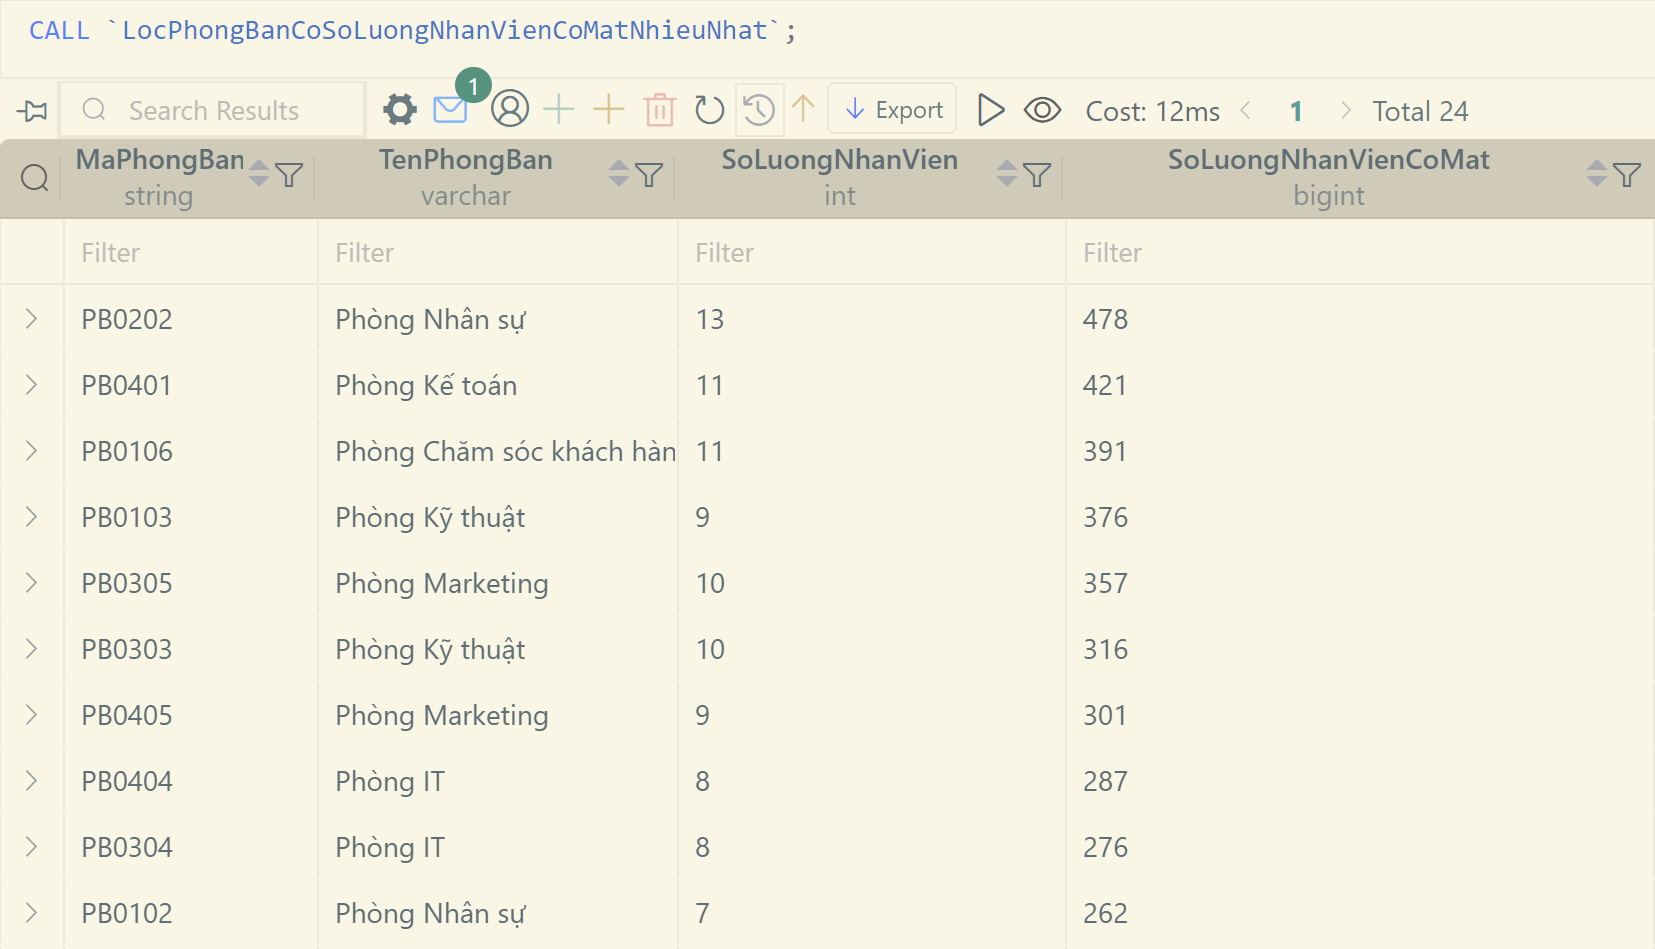
\includegraphics[width=0.8\linewidth]{content/images/procedure_1.png}
    \caption{Kết quả sau khi thực thi thủ tục LocPhongBanCoSoLuongNhanVienCoMatNhieuNhat}
    \label{fig:procedure_1}
\end{figure}

\newpage
\subsubsection{Thủ tục 2}
\textbf{Mô tả thủ tục:} Thủ tục dùng để lọc ra các phòng ban có số lượng nhân viên lớn hơn một con số được người dùng nhập vào.

\textbf{Input:}
\begin{itemize}
    \item [--] tham số minEmployeeCount, có kiểu \texttt{INT}
\end{itemize}

\textbf{Output:} Bảng thông tin của các phòng ban có số lượng nhân viên lớn hơn tham số được truyền vào.

\textbf{Câu lệnh tạo thủ tục}
\begin{minted}{mysql}
--Lọc phòng ban có số lượng nhân viên lớn hơn số lượng cho trước
CREATE PROCEDURE LocPhongBanCoSoLuongNhanVienLonHon(IN minEmployeeCount INT)
BEGIN
    SELECT 
        PB.TenPhongBan, COUNT(NV.MaNV) AS EmployeeCount
    FROM 
        PhongBan PB
    LEFT JOIN 
        NhanVien NV ON PB.MaPhongBan = NV.MaPhongBan
    WHERE 
        PB.SoLuongNhanVien > minEmployeeCount
    GROUP BY 
        PB.TenPhongBan
    HAVING 
        EmployeeCount > minEmployeeCount
    ORDER BY 
        EmployeeCount DESC;
END//
\end{minted}

\textbf{Kết quả:} 
\begin{figure}[H]
    \centering
    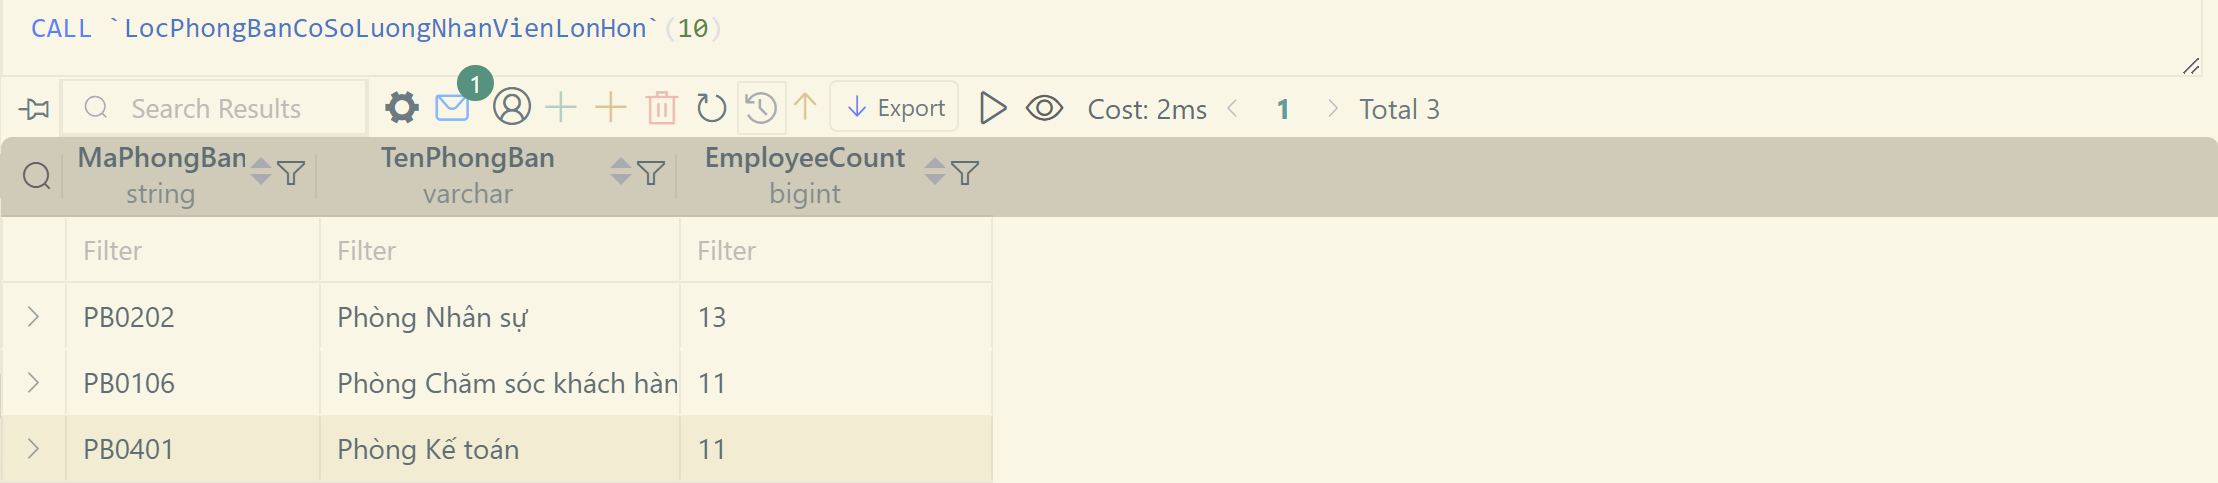
\includegraphics[width=\linewidth]{content/images/procedure_2.png}
    \caption{Kết quả sau khi thực thi thủ tục LocPhongBanCoSoLuongNhanVienLonHon với số lượng nhân viên tối thiểu là 10}
    \label{fig:procedure_2}
\end{figure}
\newpage